
\begin{comment}
\begin{figure}
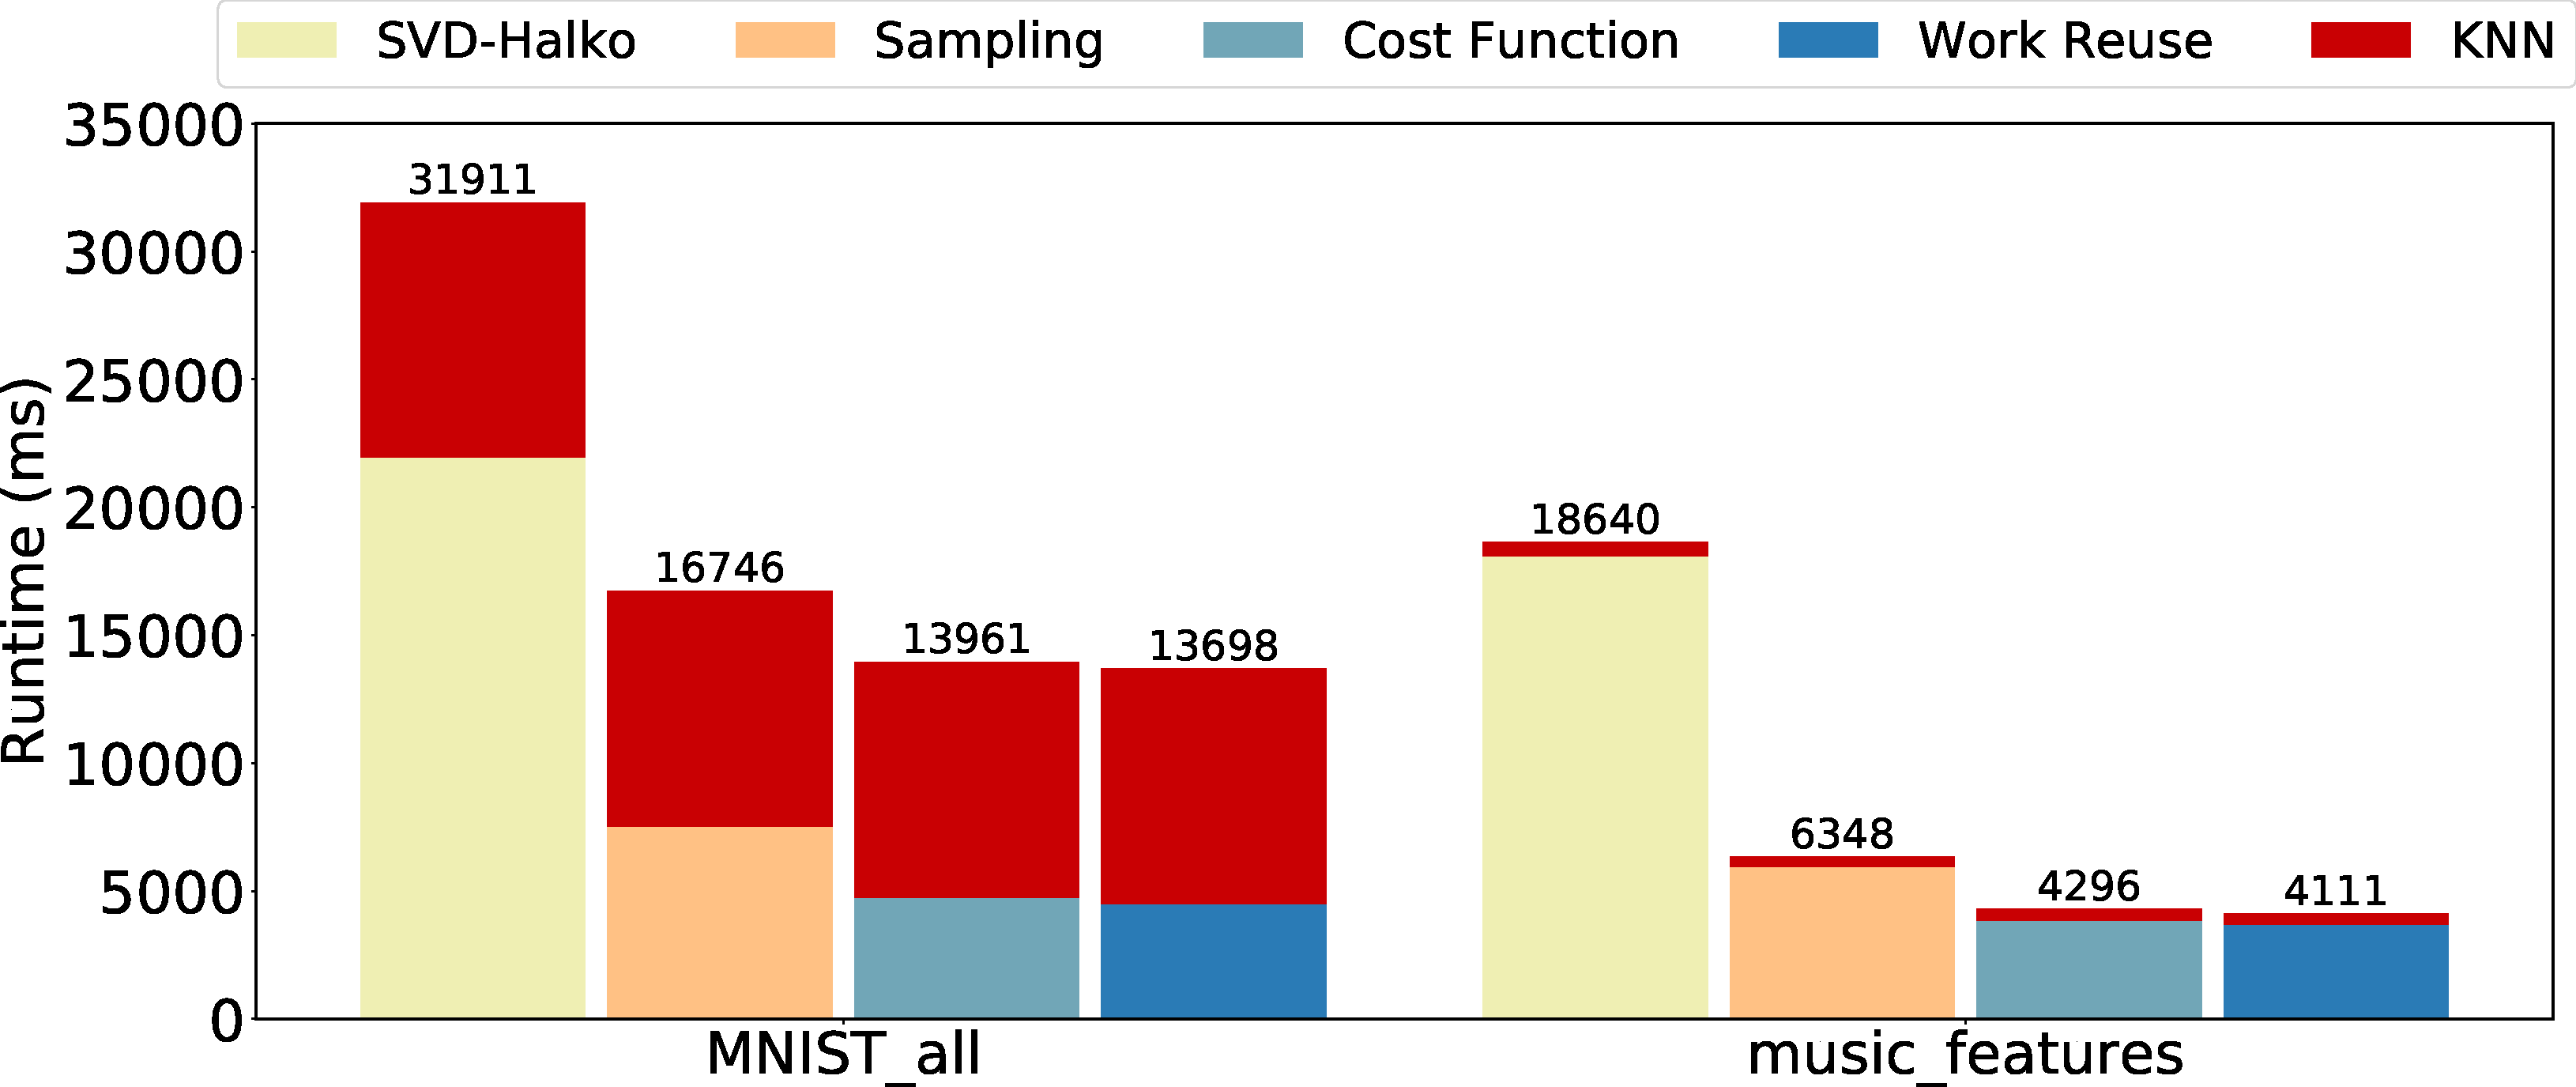
\includegraphics[width=\linewidth]{figs/beyond_tss_lesion.pdf}
\caption[]{End-to-End runtime lesion study of the entire MNIST dataset and the FMA featurized music dataset. Each of DROP's contributions provides a runtime improvement.}
\label{fig:beyond_lesion}
\end{figure}
\end{comment}



\section{Conclusion}
\label{sec:conclusion}

Advanced data analytics techniques must scale to rising data volumes. 
DR techniques offer a powerful toolkit when processing these datasets, with PCA frequently outperforming popular techniques in exchange for high computational cost. 
In response, we propose DROP, a new dimensionality reduction optimizer. 
DROP combines progressive sampling, progress estimation, and online aggregation to identify high quality low dimensional bases via PCA without processing the entire dataset by balancing the runtime of downstream tasks and achieved dimensionality. 
Thus, DROP provides a first step in bridging the gap between quality and efficiency in end-to-end DR for downstream \red{analytics}. 

%We revisit canonical operators for time series dimensionality reduction and the measurement study of~\cite{keogh-study}, and show that PCA is more effective than popular alternatives in the data mining literature often by a margin of over $2\times$ on average on gold-standard time series benchmark data sets with respect to output data dimension. More surprisingly, we empirically demonstrate that a small number of samples are sufficient to accurately characterize directions of maximum variance and obtain a high-quality low-dimensional transformation.


